\section*{1}

\subsection*{a}
As in slides from last semester.
We just have to replace C with S and v with w.

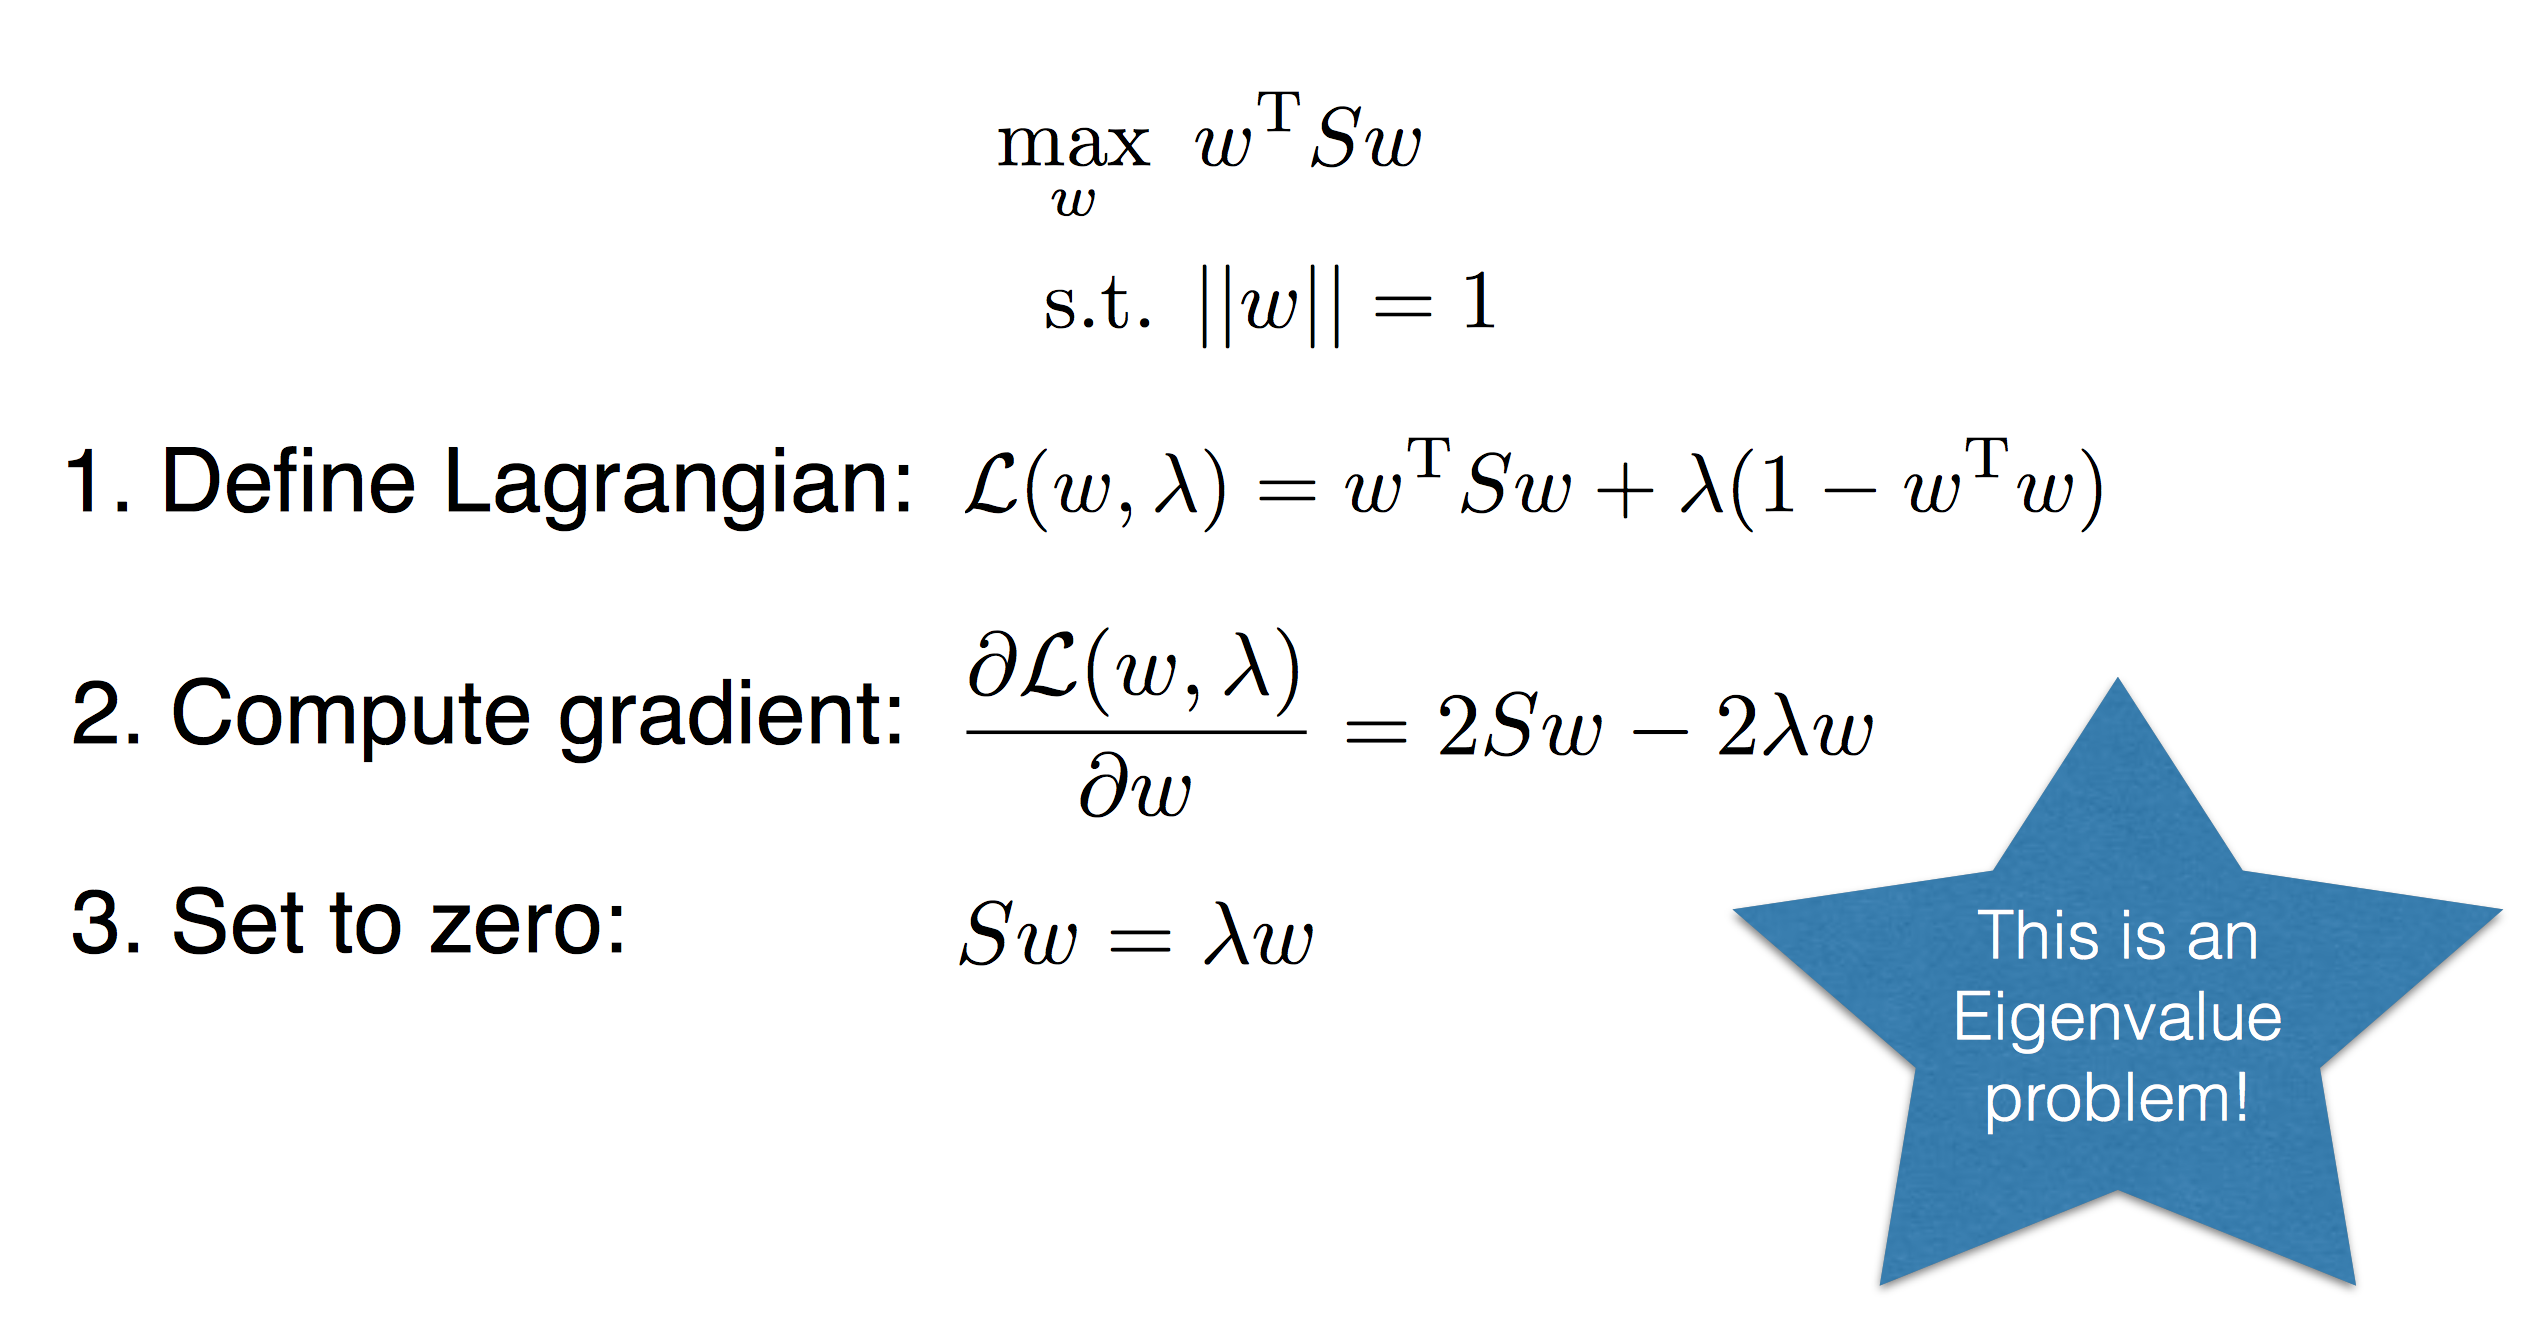
\includegraphics[scale=0.3]{1aEx6.png}

\subsection*{b}
\begin{gather*}
C = \sum_{i=1}^N \phi (x_i) \phi (x_i)^T \\
K_{ij} = \phi (x_i)^T \cdot \phi (x_j) \\
PCA: C v = \lambda v \\ 
\end{gather*}
Show: $K \alpha = \lambda \alpha$, where $v = \phi^T \alpha$, $\Phi = [\phi(x_i) ... \phi(x_n)]$

\begin{gather*}
C v = \lambda v \\
(\sum_{i=1}^N \phi(x_i) \phi(x_i)^T) \cdot \Phi^T \alpha = \lambda \cdot \Phi^T \alpha \\
(\Phi \Phi^T)^{(-1)} (\sum_{i=1}^N \phi (x_i) \phi (x_i)^T) \cdot \Phi^T \alpha = \lambda \alpha \\
\end{gather*}


